\documentclass[10pt]{article}
\usepackage[CJKchecksingle,CJKnumber]{xeCJK}
\setCJKmainfont[BoldFont={Adobe Heiti Std},
    ItalicFont={Adobe Kaiti Std}]{Adobe Song Std}
\setCJKsansfont{Adobe Heiti Std}
\setCJKmonofont{Adobe Fangsong Std}
\punctstyle{hangmobanjiao}
\usepackage{graphicx}
\usepackage{fancyhdr}
\usepackage{amsfonts}
\usepackage{booktabs}
\usepackage[svgnames, table]{xcolor}
\usepackage[bookmarksnumbered, pdfencoding=auto, pdfpagelayout=TwoPageRight,
breaklinks, colorlinks, linkcolor=blue, urlcolor=blue]{hyperref}
\usepackage{subfig}
\newcommand{\Original}{\fontsize{25pt}{\baselineskip}\selectfont}
\linespread{1.4}
\setlength{\parskip}{0.5\baselineskip}
\renewcommand{\contentsname}{目录}
\renewcommand{\figurename}{图}
\renewcommand{\refname}{参考文献}
\renewcommand{\figureautorefname}{图}
\pagestyle{fancy}
\begin{document}\large
\title{\Original{大实验开题报告}}
\author{刘玟彤\quad 学号: 2015011254 \\ 王诗媛\quad 学号:2015011483 \\ 徐禹生 \quad 学号:2015011244}

\maketitle

\section{实验内容}
\subsection{实验任务}
\begin{enumerate}
\item 实现支持指令流水的CPU
\item 使用基本存储和扩展存储以及输入/输出
\item 进行扩展
\end{enumerate}
\subsection{实验目标}
\begin{enumerate}
\item 能运行监控程序, 并在监控程序中运行PROJECT 1的程序
\item 能运行Ucore,并在Ucore下运行应用程序
\item 有可供演示的应用程序
\end{enumerate}
\subsection{实现指令}
除了基础指令之外,我们组还要实现的指令包括:
\begin{enumerate}
\item NEG
\item SLTI
\item SW\_RS
\item SRLV
\item NOT
\end{enumerate}
\subsection{扩展方案}
\begin{enumerate}
\item 对流水线进行完善,解决结构冲突、数据冲突和控制冲突,并实现对冲突的检测
\item 实现软件中断
\item 实现双机通信,通过串口来完成
\item 连接VGA和PS/2键盘这些外设,以便更好地控制和展示
\end{enumerate}
\subsection{展示方案}
在没有连接VGA和键盘的情况下,可以通过串口传输数据进行展示。在连接VGA和键盘之后,可以从键盘输入,从VGA显示结果。

\section{实验设计}
\subsection{数据通路}
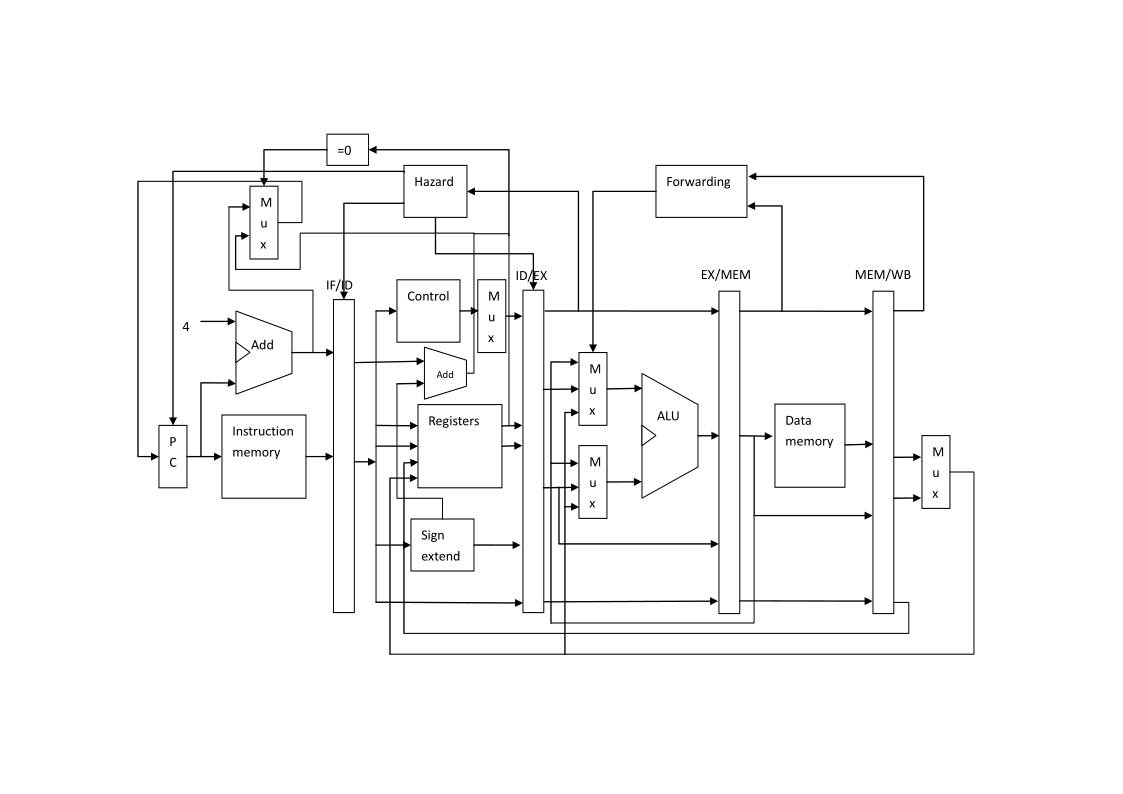
\includegraphics[scale = 0.5]{数据通路.png}
\subsection{五级流水结构}
采用经典的五级流水结构,包括IF(取指),ID(译码),EXE(计算),MEM(访存)和WB(写回)五个阶段。
\end{document}
